\documentclass[a4paper]{article}

%sinuit
\usepackage{siunitx}
%image insertion
\usepackage{graphicx} %image settings
\DeclareGraphicsExtensions{.pdf,.png,.jpg}

%math
\usepackage{amsmath} %math
%\usepackage{cmbright} %math font

%font
\usepackage{kotex}
\usepackage{fontspec}
\ifx가가
\setmainhangulfont[Ligatures=TeX,
BoldFont={KoPubBatang Medium}]{KoPubBatang Light}
\setsanshangulfont[Ligatures=TeX,
BoldFont={KoPubDotum Medium}]{KoPubDotum Light}
\setmainhanjafont[Ligatures=TeX,
BoldFont={KoPubBatang Medium}]{KoPubBatang Light}
\setsanshanjafont[Ligatures=TeX,
BoldFont={KoPubDotum Medium}]{KoPubDotum Light}
\xetexkofontregime[puncts=prevfont, colons=prevfont, cjksymbols=hangul]{latin}
\fi

%줄간격
\usepackage{setspace}
%\usepackage{indentfirst}
\setstretch{1.3}
\everydisplay{\setstretch{1.2}}

%subfigure
\usepackage{subfigure}

\pagestyle{plain}
\title{물리 실험보고서 1}
\author{이한빈, 의예과 2016-13347}

\begin{document}


\numberwithin{equation}{section}
\maketitle

\section{Introduction}
	폐회로가 주어졌을 때 회로 내부를 지나가는 자기선속이 변하면 크기는 시간당 변화량에 비례하며 방향은 자기선속 변화의 반대인 기전력이 회로에 유도된다.
	이를 페러데이의 법칙이라고 하며 다음과 같이 표현된다.
	\begin{equation} \label{faraday}
		\epsilon = -\frac{d\Phi}{dt} 
	\end{equation}
	여기서 기전력의 방향이 자기선속 변화의 반대라는 사실을 렌츠의 법칙이라고 부른다.

	페러데이의 법칙을 이용하면 그림과 같은 전동기에서 발생하는 기전력을 계산할 수 있다.
	회로의 면적을 $A$, 회전각속력을 $\omega$, 회로가 놓여진 공간의 자기장을 $B$라고 하자.
	\begin{figure}[h] 
		\centering 
		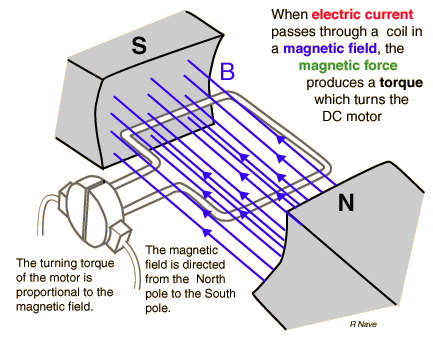
\includegraphics[width=0.4\textwidth]{img/motor.png}
		\caption{전동기}
		\label{fig:motor}
	\end{figure}
	처음에 자기장과 면벡터가 나란하면 시간에 따른 자기선속은 다음과 같다.
	\begin{equation} \label{line}
		\Phi = \vec{A} \cdot \vec{B} = AB\cos{}\omega{}t
	\end{equation} 

	식 (\ref{faraday})과 식 (\ref{line})으로부터 전동기에서 발생하는 기전력을 구하면 다음과 같다.
	\begin{equation}
		\epsilon = -\frac{d\Phi}{dt} = AB\omega{}\sin{}\omega{}t
	\end{equation}

	따라서 일정한 속력으로 회전하는 전동기에서 발생하는 기전력은 사인파의 형태로 나타남을 알 수 있다.
	반대로 전류가 흐르는 폐회로는 자기장에서 토크를 받는다.
	장치가 전동기와 동일하게 되어있다고 가정하고 회로에 전류 $I$가 흐른다고 하자.
	회로의 자기모멘트는 다음으로 주어진다.
	\begin{equation}
		\vec{\mu} = I\vec{A}
	\end{equation}

	회로가 받는 토크는 자기모멘트와 자기장의 외적이므로 폐회로가 받는 토크는 다음과 같다.
	\begin{equation} \label{eq:osc}
		|\vec{\tau}| = |\vec{\mu} \times \vec{B}| = IAB\sin{\omega{}t}
	\end{equation}

 	전동기에서 직류전원을 연결하면 식 (\ref{eq:osc})에서 볼 수 있듯이 전동기가 지속적으로 같은 방향으로 회전하지 않고 진동하는 것을 알 수 있다.
 	이를 극복하기 위해 회로에 흐르는 전류의 방향을 지속적으로 바꾸는 장치를 정류자라고 한다.
 	\begin{figure}[h]   		
 		\centering
 		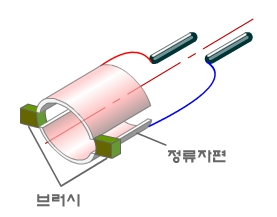
\includegraphics[scale=0.5]{img/a-5385.jpg}
 		\caption{2단 정류자}
   		\label{fig:com}
 	\end{figure}

 	그림 \ref{fig:com}의 정류자는 전류의 방향이 $\ang{180;;}$마다 역전되므로 회로가 받는 토크는 원래토크에서 절댓값이 씌어진 형태가 된다.
 	기전력이 유도되는 상황에서도 마찬가지로 기전력은 절댓값이 씌어진 다음과 같은 형태로 주어진다.
 	\begin{equation}
 		|\epsilon| = AB\omega{}|\sin{\omega t}|
 	\end{equation}

 	본 실험에서는 첫 번째로 솔레노이드와 막대자석을 이용하여 렌츠의 법칙을 검증한다.
 	두 번째로는 전동기에 연결된 회로를 균일한 자기장 속에서 회전 시켰을 때 유도되는 기전력을 측정하여 렌츠의 법칙과 페러데이의 법칙을 검증한다.
 	또 전동기의 AC, DC출력 단자에 대해 각각 실험하고 비교함으로써 정류자의 효과에 대해서도 알아봤다.
	\newpage

	\section{Method}
	\subsection{렌츠의 법칙 확인}
	준비물 : 막대자석, 솔레노이드, 오실로스코프
	솔레노이드의 양 극을 오실로스코프에 연결했다. 
	그 후 N극을 솔레노이드 내부에 넣은 상태로 당길 때 오실로스코프로 측정된 기전력의 방향을 얻었다.
	당기는 대신 N극을 집어 넣을 때 오실로스코프로 측정한 기전력의 방향을 얻었다.
	위 과정을 N극 대신 S극으로 반복했다.

	\begin{figure}[h]
		\centering
		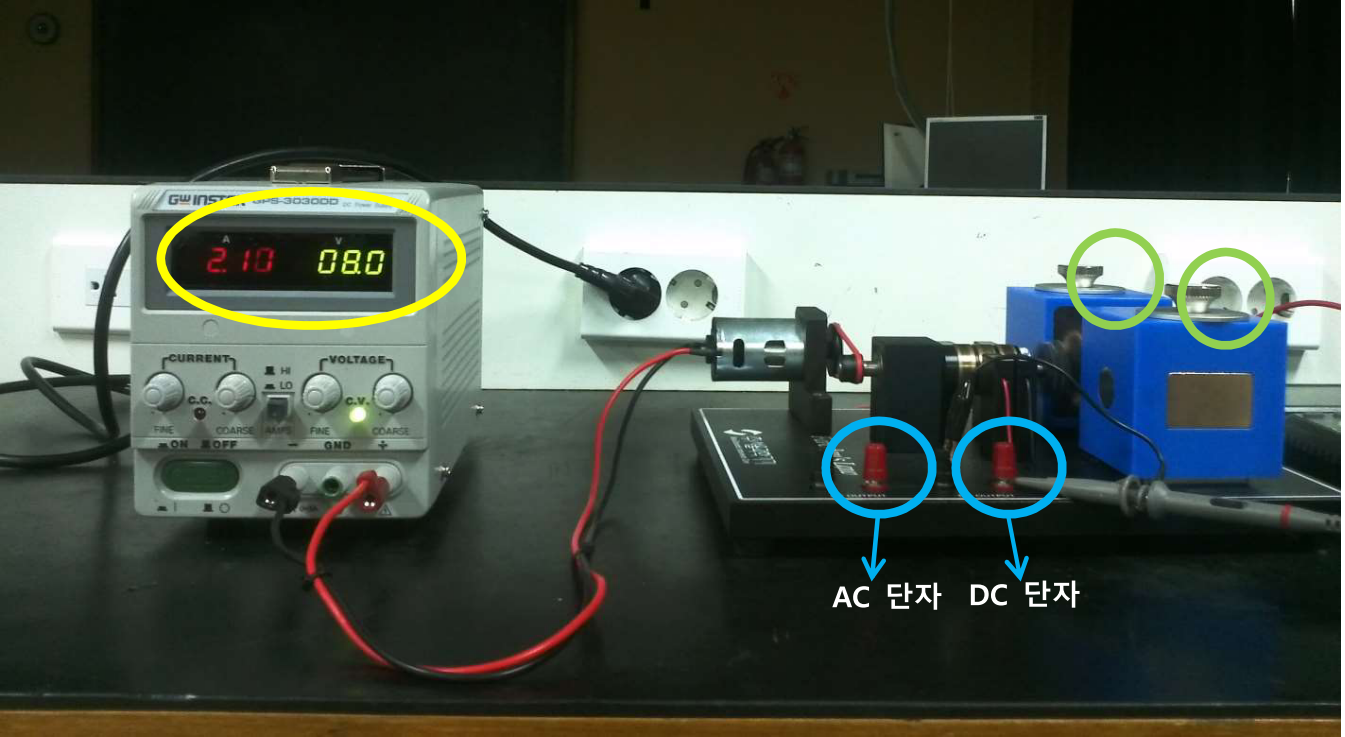
\includegraphics[width=0.7\textwidth]{img/exp1.PNG}
		\label{fig:exp1}
		\caption{Faraday 실험장치}
	\end{figure}
	
	\subsection{Faraday 실험장치 AC 출력}
	준비물: Faraday 실험장치, 전동기, 직류입력장치
	오실로스코프를 Faraday 실험장치의 AC단자에 연결한다. 직류전원장치를 Faraday 실험장치에 연결하고 전류와 전압을 
	\subsection{Faraday 실험장치 DC 출력}
	준비물: Faraday 실험장치, 전동기, 직류입력장치






\section{Reference}
	1. Halliday, D., Resnick, R., \& Walker, J. (2014). {\it{}Principles of Physics} (10th ed., Vol. 2). Hoboken, NJ: Wiley. 

\end{document} 

%실험에서 개선할 점 등 피피티에서 봤던 거 모두 적어서 처리합시다